\chapter{Opis projektu}
\thispagestyle{chapterBeginStyle}

\iffalse
{\color{dgray}
W tym rozdziale przedstawiono szczegółowy projekt systemy w notacji UML uwzględniający wymagania funkcjonalne opisane w rozdziale~\ref{rozdzial1}. Do opisu relacji pomiędzy składowymi systemu wykorzystano diagramy \ldots.
Przedstawiono w pseudokodzie i omówiono algorytmy generowania \ldots.
}


\section{Grupy użytkowników i założenia}

{\color{dgray}
Architektura systemu \ldots jest wielowarstwowa i rozproszona, przy czym \ldots. Podsystem  \ldots jest systemem zbiorczym dla danych \ldots wysyłanych do serwera \ldots. 

Taka architektura jest zgodna z wzorcem projektowym MVC\footnote{Należy odnieść się do wykorzystywanych wzorców projektowych} (ang.  Model-View-Controller). Przetwarzanie danych odbywa się \ldots.
} 

\section{Przypadki użycia i scenariusze}

W tej sekcji należy przedstawić przypadki użycia oraz odpowiadające im scenariusze dla poszczególnych grup użytkowników \ldots.

\section{Diagramy klas}

W tej sekcji należy przedstawić diagramy klas dla odpowiednich elementów systemu zidentyfikowane na podstawie wcześniejszych rozważań 

\section{Diagramy aktywności}

W tej sekcji należy przedstawić diagramy aktywności dla elementów systemu i odpowiednich procesów wynikające z wcześniejszej analizy.  

{\color{dgray}
W niniejszym rozdziale przedstawiono diagramy aktywności \ldots. Diagram na rysunku~\ref{czynnosci_GD} przedstawia \ldots.
} 

\begin{figure}[h!]
\begin{center}
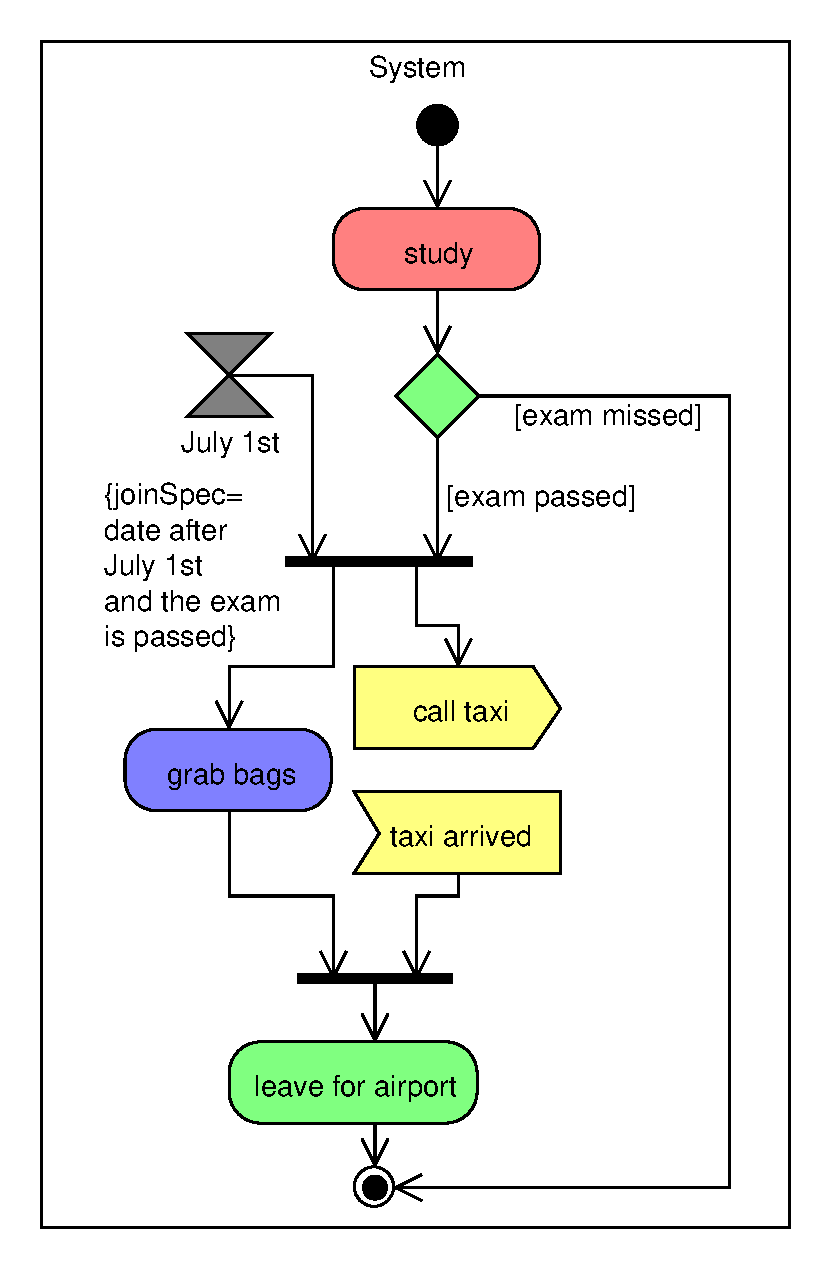
\includegraphics[width=0.5\textwidth]{aktyw.pdf}
\end{center}
\caption{{\color{dgray}Diagram aktywności związany z procesem rejestracji dokumentu.}} \label{czynnosci_GD}
\end{figure}  

\section{Diagramy sekwencji}

W tej sekcji należy przedstawić diagramy sekwencji dla obiektów systemu zidentyfikowanych na podstawie wcześniejszych rozważań. Należy wykorzystać nazewnictwo wprowadzone w poprzednich rozdziałach, w szczególności odpowiadające definicjom wprowadzonych klas.

\section{Diagramy stanów}

W tej sekcji należy przedstawić diagramy stanów w których może znaleźć się system. Diagramy te są szczególnie istotne przy projektowaniu systemów czasu rzeczywistego. 

\section{Projekt bazy danych}

W tej sekcji należy przedstawić projekt bazy danych. Należy omówić wycinek rzeczywistości i odpowiadające mu zidentyfikowane elementy systemu, których wartości będą podlegać utrwalaniu. Należy przedyskutować wybór typów danych dla atrybutów poszczególnych obiektów. Należy uzasadnić wybór platformy DBMS. Dla relacyjnych baz danych należy przedyskutować jej normalizację.

\section{Opis protokołów}

W tej sekcji należy omówić protokoły wykorzystywane przez komponenty systemu. Omówić formaty komunikatów i zilustrować je przykładami. 

\section{Opis algorytmów}

W tej sekcji należy wymienić i przedyskutować algorytmy wykorzystywane w systemie. Algorytmy należy przedstawić w pseudokodzie (wykorzystać pakiet \texttt{algorithm2e}). Omówienia poszczególnych kroków algorytmów powinny zawierać odwołania do odpowiednich linii pseudokodu. Dla zaproponowanych autorskich algorytmów należy przeprowadzić analizę ich złożoności czasowej i pamięciowej. 

{\color{dgray}
Algorytm bąblowania jest przedstawiony w Pseudokodzie~\ref{alg:mine}.
}

{\small
\begin{pseudokod}[H]
%\SetAlTitleFnt{small}
\SetArgSty{normalfont}
\SetKwFunction{Process}{Process}
\SetKwFunction{Calculate}{Calculate}
\KwIn{Zbiór bąbli $B$}
\KwOut{Wyporność $W$}
\ForEach{$b \in B$}{
\Process{$b$}\;
\For{$i \leftarrow 1$ \KwTo $|B|$}{
\If{\Calculate{EW($i$,$b$)} $\le$ 0}{
$b \leftarrow 2*b$\;
}
}
}
\While{$B \neq \emptyset$}{
\For{$j \leftarrow 1$ \KwTo $|B|$}{
\If{\Calculate{FT($j$,$\hat{b}$)} $\le 0$}{
$w \leftarrow 2*\hat{b}$\;
$W \leftarrow W \cup \{w\}$\;
$B \leftarrow B \setminus \{b\}$\;
}
}
}
\caption{Wyporność przez bąblowanie}\label{alg:mine}
\end{pseudokod}
}


W tym rozdziale opisane są wszystkie elementy pamięci maszyny. Zmienne reprezentujące elementy pamięci maszyny są zmiennymi globalnymi. Cała pamięć jest czyszczona (nie licząc części kodu) przed rozpoczęciem wykonywania każdego zapytania.

\section{Komórka pamięci}

Komórka pamięci to podstawowa składowa wielu elementów pamięci. Każda komórka ma jeden z dwóch typów. Komórka zmiennej zawiera tag, który może być {REF} lub {STR}, a także adres dowolnej innej komórki znajdującej się w pamięci. Komórka funktora zawiera reprezentację funktora $f/n$, gdzie $f$ jest nazwą funktora, a $n$ liczbą argumentów przez niego przyjmowanych. Domyślnie każda komórka jest komórką zmiennej o tagu {REF} i adresie pokazującym na samą siebie, czyli tzw. komórką nieprzypisaną. Nieprzypisana komórka odpowiada nieprzypisanej zmiennej.\\
W implementacji komórka jest reprezentowana przez własną klasę z polami \texttt{string tag} i \texttt{shared\_ptr<Address> addr}.

\section{\texttt{HEAP} - Sterta}

Sterta to główny blok pamięci w którym przechowywane są komórki pamięci reprezentujące struktury i zmienne (w przeciwieństwie do rejestrów, w których wszystkie komórki są komórkami REF z adresami komórek ze sterty). Adres końca sterty jest pamiętany przez rejestr H. Rejestr H jest aktualizowany na końcu każdej instrukcji, która dodaje nowe komórki do sterty.\\
Sterta jest reprezentowana przez klasę \texttt{MemoryBloc}, która trzyma komórki w werktorze z przeładowanymi operatorami dostępu, które w przypadku próby dostępu do komórki o indeksie większym od długości wektora najpierw zapełnia brakujące pola nieprzypisanymi komórkami. Rejestr H jest reprezentowany przez liczbę naturalną równą długości sterty.

\section{Rejestry tymczasowe}

Rejestry zawierają komórki z adresami pokazującymi na stertę. Komórki w rejestrach służą jako wskaźniki do miejsc w stercie gdzie przechowywane są podtermy zawarte w obecnie ewaluowanym termie. Rejestry tymczasowe przestają być użyteczne po przejściu do następnego termu i są nadpisywane. Rejestry tymczasowe są przypisywane do podtermów przez kompilator.\\
Rejestry tymczasowe są reprezentowane przez klasę \texttt{MemoryBloc}, tak samo jak sterta.

\section{Rejestry argumentów}

Rejestry argumentów tak samo jak rejestry tymczasowe zawierają komórki będące wskaźnikami na stertę. Przechowują one adresy argumentów, czyli bezpośrednich podtermów ewaluowanego termu i służą do przekazywania argumentów przy wywołaniu instrukcji \texttt{call}. Są one ustawiane w trakcie ewaluowania termu z zapytania i są one wczytywane do innych rejestrów w trakcie dopasowywania do głowy klauzuli.\\
Rejestry argumentów są reprezentowane przez klasę \texttt{MemoryBloc}.

\section{Rejestry trwałe}

Rejestry trwałe działają podobnie do rejestrów tymczasowych i rejestrów argumentów i służą do pamiętania zmiennych pojawiających się w wielu termach w zapytaniu lub regule. Rejestry trwałe są zapisywane w środowiskach i są wymieniane wraz ze zmianą aktywnego środowiska. Te rejestry są przydzielane do zmiennych przez kompilator.\\
Rejestry argumentów są reprezentowane przez klasę \texttt{MemoryBloc}.

\section{\texttt{MODE} - Tryb maszyny}

W momencie wykonywania zapytania maszyna w każdym momencie może być w jednym z dwóch trybów: $read$ i $write$. Tryb jest ustawiany przez instrukcję \texttt{get\_structure} i zmienia działanie instrukcji \texttt{unify\_variable} i \texttt{unify\_value}. Drugim rejestrem globalnym używanym tylko przez te instrukcje jest rejestr \texttt{S} przechowujący adres w stercie.\\
Zarówno \texttt{MODE} i \texttt{S} reprezentowane są przez liczby naturalne, przy czym $mode$ może być w tylko dwóch stanach: 0 ($write$) i 1 ($read$). 

\section{\texttt{CODE} - Magazyn kodu}

W magazynie kodu przechowywana jest załadowana lista instrukcji wygenerowana przez kompilator lub pobrana z pliku. Instrukcje programu i zapytanie ładowane są osobno przed rozpoczęciem wykonywania zapytania. Najpierw ładowane są klauzule wbudowane, które funkcjonują jak część programu, która jest niewidoczna w ładowanym pliku. Następnie ładuje program. Wszystkie etykiety są usuwane z kodu i pamiętane są osobno razem z numerami instrukcji następujących po nich. Na końcu ładowany jest kod zapytania i ustawiany jest rejestr \texttt{P} oznaczajacy miejsce w kodzie instrukcji obecnie wykonywanej i rejestr \texttt{CP} oznaczający miejsce w kodzie do którego maszyna ma wrócić po wywołaniu \texttt{proceed} lub \texttt{deallocate}. Rejestr \texttt{P} ustawiany jest na pierwszą instrukcję z zapytania, a \texttt{CP} na koniec kodu.\\
Magazyn kodu jest reprezentowany przez wektor wektorów stringów, gdzie każde pole zawiera osobno nazwę instrukcji i wszystkie argumenty jako stringi. Etykiety są pamiętane w \texttt{std::unordered\_map} gdzie kluczem jest string będący nazwą etykiety, a warotścią jest liczba naturalna oznaczająca indeks instrukcji której odpowiada etykieta. Rejestry \texttt{P} i \texttt{CP} są reprezentowane przez liczby naturalne.

\section{\texttt{TRAIL} - Ślad}

Ślad służy do zapamiętywania kiedy nieprzypisane zmienne zostają przypisane tak, żeby w przypadku nawrotu dało się cofnąć odpowiednie przypisania. Przechowuje on adresy zmiennych w kolejności, w której zostają przypisane. Nowy element zostaje dodany na koniec śladu za każdym razem gdy zostaje wywołana operacja $bind$. W przypadku nawrotu i konieczności odłączania zmiennych rejestr \texttt{HB} pamięta wielkość sterty przed ostatnim punktem wyboru, żeby nie próbować odłączać zmiennych usuniętych przez nawrót.\\
Ślad jest reprezentowany przez wektor adresów przypisywanych komórek. Podczas nawrotu odpowiednia ilość elementów z końca śladu jest usuwana. Rejestr \texttt{HB} jest reprezentowany przez liczbę naturalną oznaczającą ilość komórek w stercie.

\section{\texttt{AND-STACK} i \texttt{OR-STACK} - Stosy}

\texttt{AND-STACK} jest stosem przechowującym środowiska. Środowisko przechowuje rejestry trwałe i punkt powrotu (\texttt{CP}) dla obecnie przetwarzanego zapytania lub reguły, a także indeks poprzedniego środowiska, które ponownie się uaktywni po dealokacji obecnego. Globalny rejestr \texttt{E} zawiera indeks obecnie aktywnego środowiska. \texttt{OR-STACK} jest stosem przechowującym punkty wyboru. Punkt wyboru zapamiętuje moment w którym maszyna dokonuje wyboru, w jaki sposób próbować udowodnić term z zapytania lub ciała reguły. W przypadku Niepowodzenia w ewaluacji maszyna wraca do ostatniego punktu wyboru i próbuje udowodnić term w inny sposób. Punkt wyboru przechowuje wartości wielu globalnych rejestrów w momenie jego utworzenia: \texttt{E}, \texttt{CP}, \texttt{B}, \texttt{H}. Oprócz tego punkt wyboru w momencie utworzenia zapamiętuje też długość śladu, rejestry argumentów (których ilość jest pamiętana w globalnym rejestrze \texttt{num\_of\_args} i numer instrukcji do której maszyna ma przejść w przypdaku konieczności powrotu do tego punktu. Każdy punkt wyboru chroni środowiska istniejące w momencie jego utworzenia przed usunięciem po dealokacji w razie konieczności ponownej aktywacji tego środowiska po nawrocie. Alternatywną metodą implementacji jest przechowywanie środowisk i punktów wyboru na jednym stosie \cite{WAM}. Wtedy każdy punkt wyboru chroni przed usunięciem wszystkie środowiska pod nim na stosie i globalny rejestr \texttt{B} pamięta indeks na stosie aktywnego punktu wyboru. Ze względu na łatwość w implementacji zdecydowałem się na użycie dwóch stosów, a rejestr \texttt{B} służy do ochrony środowisk pamiętając aktywne środowisko w momencie utworzenia ostatniego punktu wyboru.\\
Oba stosy są reprezentowane przez wektory. Środowisko jest reprezentowane przez własną klasę z polami przechowującymi warotści rejestrów trwałych i rejestrów \texttt{E} i \texttt{CP}. W trakcie przełączania aktywnego środowiska wartości rejestrów trwałych są zapisywane w poprzednim środowisku, a na ich miejsce są wczytywane rejestry trwałe z nowego środowiska. Punkt wybory też jest reprezentowany przez własną klasę z polami \texttt{E}, \texttt{CP}, \texttt{B}, \texttt{H}, \texttt{TR} (długość śladu), \texttt{BP} (instrukcja do wykonania po nawrocie). Wszystkie te pola są liczbami naturalnymi.
\fi

Sposób działania opisanej implementacji jest oparty na sposobie działania SWI-Prologa z dodatkową możliwością używania kompilatora i maszyny WAM oddzielnie. Założeniem było zaimplementowanie podstawowej funkcjonalności SWI-Prologa, dając także lepszy wgląd w działanie WAM poprzez danie użytkownikowi możliwości uzyskania tekstowej reprezentacji kodu Prologa skompilowanego do listy instrukcji WAM, a następnie uruchomienia WAM dla tych instrukcji (lub napisanych ręcznie przez użytkownika). Do tego celu zawarte w aplikacji implementacja WAM i kompilator są dwiema łatwo rozróżnialnymi częściami uruchamianymi z głównej pętli aplikacji i możliwymi do uruchomienia osobno. W celu dalszej rozbudowy funkcjonalności i umożliwieniu analizy efektywności w projekcie implementacji znalazły się też dodatkowe instrukcje nie znajdujące się w zestawie instrukcji WAM dla czystego języka Prolog, wbudowane predykaty i wbudowana opcja pomiaru czasu i liczby inferencji.

\section{Dodatkowa funkcjonalność}

Zaproponowana implementacja zawiera wbudowane predykaty: \texttt{=/2}, \texttt{write/1}, \texttt{nl/0}, \texttt{./2} oraz \texttt{</2}. Ich kod zawsze jest dołączany na początek strefy kodu WAM przed kodem programu.\\
Predykat \texttt{=/2} unifikuje oba argumenty, tak jak w SWI-Prologu i jest zaimplementowany ze względu na wygodę użytkowania.\\
Predykat \texttt{write/1} wypisuje tekstową reprezentację termu z argumentu na standardowe wyjście. Działa rekurencyjnie dla termów złożonych i wypisuje też listy w opdowiedni sposób. Dla nieprzypisanych zmiennych wypisuje ich adres w pamięci.\\
Predykat \texttt{nl/0} wypisuje na standardowe wyjście nową linię.\\
Term \texttt{.(A,B)} reprzezentuje listę \texttt{B} z dołączonym pierwszym elementem \texttt{A}. Pustą listę oznacza term \texttt{[]}. Predykat \texttt{./2} sprawdza czy term jest poprawną reprezentacją listy, tzn. czy drugi argument jest poprawną reprezentacją listy (w tym może być pustą listą).\\
Predykat \texttt{</2} sprawdza czy oba argumenty są liczbami całkowitymi i czy pierwszy argument jest mniejjszy od drugiego.\\

Do implementacji części z tych predykatów wymagana była implementacja specjalnych instrukcji, które nie są nigdy generowane przez kompilator ale pojawiają się w kodzie wbudowanych predykatów, żeby umożliowić ich funkcjonalność nie dostępną dla czystego Prologa. Instrukcje \texttt{write}, \texttt{nl}, \texttt{less\_than} uruchamiają funkcjonalność odpowiadających im predykatom dla odpowiednich rejestrów argumentów.\\

Przy uruchomieniu aplikacji dodatkowo jest dostępny tryb drukowania statystyk. W trakcie wykonywania każdego zapytania mierzony jest czas i liczba inferencji.\\

\section{Kompilacja}

Ważnym elementem implementacji jest kompilator. Aplikacja zawiera jeden kompilator kompilujący kod języka Prolog do tekstowej listy instrukcji WAM. Kompiluje on zarówno zapytania jak i programy. Metodą rozróżniania jest to, że zapytania w zaprzoponowanej implementacji zawsze muszą zaczynać się od \texttt{?-}.\\
Kompilator obsługuje też termy o składni nie zgodnej z czystym Prologiem:\\
\texttt{X = Y} jest kompilowane jak \texttt{=(X,Y)},\\
podobnie \texttt{X < Y} i \texttt{X > Y},\\
\texttt{[X]} oznacza listę i jest kompilowane jak \texttt{.(X,[])}, dozwolone są też listy o wielu elementach (\texttt{[X, Y, Z]}),\\
\texttt{[X | Y]} oznacza listę, której ogonem jest \texttt{Y}, także można użyć wielu elementów (\texttt{[X, Y | Z]}).

\section{Gramatyka}

Dwa mające w gramatyce tokeny to \texttt{VAR} i \texttt{STRUCT}. Oznaczają one odpowiednio nazwy zmiennych i struktur. Składają się z dowolnej kombinacji liter małych, wielkich, cyfr i podkreślników. Różnią się tym że nazwy zmiennych zaczynają się wielką literą, w przeciwieństwie do nazw struktur.\\

\newcommand{\INDSTATE}[1][1]{\STATE\hspace{#1\algorithmicindent}}

\begin{algorithm}[H]
\begin{algorithmic}
\STATE \texttt{program}\\
\INDSTATE[5] \texttt{predicates}\\
\INDSTATE[5] \texttt{?- terms .}\\
\texttt{predicates}\\	 
\INDSTATE[5] \texttt{predicates predicate}\\
\INDSTATE[5] \texttt{predicate}\\
\texttt{predicate}\\		  
\INDSTATE[5] \texttt{term :- terms .}\\
\INDSTATE[5] \texttt{term .}\\
\texttt{terms} \\		 
\INDSTATE[5] \texttt{terms , term}\\
\INDSTATE[5] \texttt{term}\\
\texttt{term}\\				  
\INDSTATE[5] \texttt{STRUCT ( terms )}\\
\INDSTATE[5] \texttt{STRUCT}\\
\INDSTATE[5] \texttt{VAR}\\
\INDSTATE[5] \texttt{term = term}\\
\INDSTATE[5] \texttt{term < term}\\
\INDSTATE[5] \texttt{term > term}\\
\INDSTATE[5] \texttt{[]}\\
\INDSTATE[5] \texttt{[ terms ]}\\
\INDSTATE[5] \texttt{[ terms $\vert$ term ]}\\
\caption{Gramatyka kompilatora}
\end{algorithmic}
\end{algorithm}